\chapter{Analyse des résultats}

\section{Métrique d'évaluation IoU}
En général, Intersection over Union (IoU) (ou indice de Jaccard) est considéré comme la métrique la plus populaire pour l'évaluation de détection d'objet. Dans le domaine de la détection d'objet, IoU est utilisé pour mesurer la similarité entre la bounding box prédit $B_{p}$ et la bounding box de la vérité terrain $B_{gt}$, en mesurant l'intersection (l'aire du chevauchement) pour $B_{p}$ et $B_{gt}$, divisé par l'aire de leur union, qui est:
$$IoU=J(B_{p}, B_{gt})=\frac{aire(B_{p} \cap B_{gt})}{aire(B_{p} \cup B_{gt})}$$
 
Comme illustré en figure \ref{fig:iou_example}:

\begin{figure}[!htbp]
\center
	\subfloat{{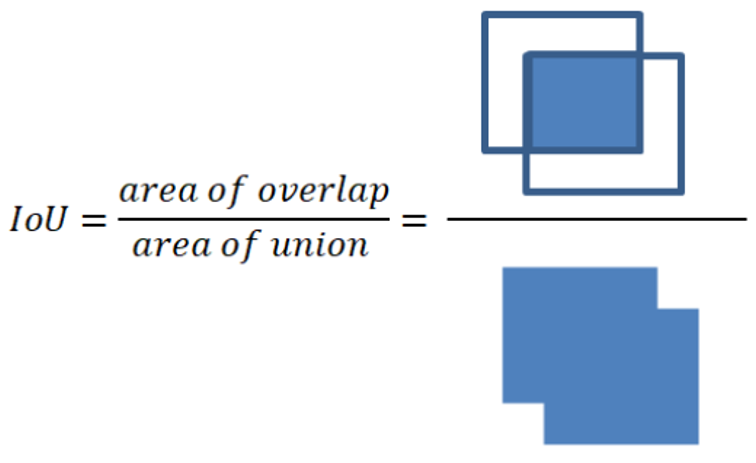
\includegraphics[scale=0.5]{IoU.png}}}
\caption{Intersection over Union (IoU)}
\label{fig:iou_example}
\end{figure}
\FloatBarrier

Dans notre cas, les bounding boxes de prédiction correspondent à la sortie de notre logiciel, ou à celle du réseau de neurone (YOLOv7). Les bounding boxes de la vérité terrain, quand à elles, correspondent à des bounding boxes annotées manuellement et qui englobe l'objet ciblé à détecter (i.e. la seiche).\\
Pour avoir la vérité terrain, nous avons utilisé LabelImg.\\
\\
Afin de classifier le résultat de la détection comme étant correcte ou non, nous comparons l'IoU à un seuil donné $T$, donc, si $IoU > T$ alors nous pouvons considérer la détection comme étant correcte, autrement, la détection est considérée comme incorrecte.\\
Dans nos testes, nous avons fixé le seuil $T$ à 0.5.

\section{Analyse et comparaison}

\clearpage